% Options for packages loaded elsewhere
\PassOptionsToPackage{unicode}{hyperref}
\PassOptionsToPackage{hyphens}{url}
\PassOptionsToPackage{dvipsnames,svgnames,x11names}{xcolor}
%
\documentclass[
  letterpaper,
  DIV=11,
  numbers=noendperiod]{scrartcl}

\usepackage{amsmath,amssymb}
\usepackage{iftex}
\ifPDFTeX
  \usepackage[T1]{fontenc}
  \usepackage[utf8]{inputenc}
  \usepackage{textcomp} % provide euro and other symbols
\else % if luatex or xetex
  \usepackage{unicode-math}
  \defaultfontfeatures{Scale=MatchLowercase}
  \defaultfontfeatures[\rmfamily]{Ligatures=TeX,Scale=1}
\fi
\usepackage{lmodern}
\ifPDFTeX\else  
    % xetex/luatex font selection
\fi
% Use upquote if available, for straight quotes in verbatim environments
\IfFileExists{upquote.sty}{\usepackage{upquote}}{}
\IfFileExists{microtype.sty}{% use microtype if available
  \usepackage[]{microtype}
  \UseMicrotypeSet[protrusion]{basicmath} % disable protrusion for tt fonts
}{}
\makeatletter
\@ifundefined{KOMAClassName}{% if non-KOMA class
  \IfFileExists{parskip.sty}{%
    \usepackage{parskip}
  }{% else
    \setlength{\parindent}{0pt}
    \setlength{\parskip}{6pt plus 2pt minus 1pt}}
}{% if KOMA class
  \KOMAoptions{parskip=half}}
\makeatother
\usepackage{xcolor}
\setlength{\emergencystretch}{3em} % prevent overfull lines
\setcounter{secnumdepth}{5}
% Make \paragraph and \subparagraph free-standing
\makeatletter
\ifx\paragraph\undefined\else
  \let\oldparagraph\paragraph
  \renewcommand{\paragraph}{
    \@ifstar
      \xxxParagraphStar
      \xxxParagraphNoStar
  }
  \newcommand{\xxxParagraphStar}[1]{\oldparagraph*{#1}\mbox{}}
  \newcommand{\xxxParagraphNoStar}[1]{\oldparagraph{#1}\mbox{}}
\fi
\ifx\subparagraph\undefined\else
  \let\oldsubparagraph\subparagraph
  \renewcommand{\subparagraph}{
    \@ifstar
      \xxxSubParagraphStar
      \xxxSubParagraphNoStar
  }
  \newcommand{\xxxSubParagraphStar}[1]{\oldsubparagraph*{#1}\mbox{}}
  \newcommand{\xxxSubParagraphNoStar}[1]{\oldsubparagraph{#1}\mbox{}}
\fi
\makeatother

\usepackage{color}
\usepackage{fancyvrb}
\newcommand{\VerbBar}{|}
\newcommand{\VERB}{\Verb[commandchars=\\\{\}]}
\DefineVerbatimEnvironment{Highlighting}{Verbatim}{commandchars=\\\{\}}
% Add ',fontsize=\small' for more characters per line
\usepackage{framed}
\definecolor{shadecolor}{RGB}{241,243,245}
\newenvironment{Shaded}{\begin{snugshade}}{\end{snugshade}}
\newcommand{\AlertTok}[1]{\textcolor[rgb]{0.68,0.00,0.00}{#1}}
\newcommand{\AnnotationTok}[1]{\textcolor[rgb]{0.37,0.37,0.37}{#1}}
\newcommand{\AttributeTok}[1]{\textcolor[rgb]{0.40,0.45,0.13}{#1}}
\newcommand{\BaseNTok}[1]{\textcolor[rgb]{0.68,0.00,0.00}{#1}}
\newcommand{\BuiltInTok}[1]{\textcolor[rgb]{0.00,0.23,0.31}{#1}}
\newcommand{\CharTok}[1]{\textcolor[rgb]{0.13,0.47,0.30}{#1}}
\newcommand{\CommentTok}[1]{\textcolor[rgb]{0.37,0.37,0.37}{#1}}
\newcommand{\CommentVarTok}[1]{\textcolor[rgb]{0.37,0.37,0.37}{\textit{#1}}}
\newcommand{\ConstantTok}[1]{\textcolor[rgb]{0.56,0.35,0.01}{#1}}
\newcommand{\ControlFlowTok}[1]{\textcolor[rgb]{0.00,0.23,0.31}{\textbf{#1}}}
\newcommand{\DataTypeTok}[1]{\textcolor[rgb]{0.68,0.00,0.00}{#1}}
\newcommand{\DecValTok}[1]{\textcolor[rgb]{0.68,0.00,0.00}{#1}}
\newcommand{\DocumentationTok}[1]{\textcolor[rgb]{0.37,0.37,0.37}{\textit{#1}}}
\newcommand{\ErrorTok}[1]{\textcolor[rgb]{0.68,0.00,0.00}{#1}}
\newcommand{\ExtensionTok}[1]{\textcolor[rgb]{0.00,0.23,0.31}{#1}}
\newcommand{\FloatTok}[1]{\textcolor[rgb]{0.68,0.00,0.00}{#1}}
\newcommand{\FunctionTok}[1]{\textcolor[rgb]{0.28,0.35,0.67}{#1}}
\newcommand{\ImportTok}[1]{\textcolor[rgb]{0.00,0.46,0.62}{#1}}
\newcommand{\InformationTok}[1]{\textcolor[rgb]{0.37,0.37,0.37}{#1}}
\newcommand{\KeywordTok}[1]{\textcolor[rgb]{0.00,0.23,0.31}{\textbf{#1}}}
\newcommand{\NormalTok}[1]{\textcolor[rgb]{0.00,0.23,0.31}{#1}}
\newcommand{\OperatorTok}[1]{\textcolor[rgb]{0.37,0.37,0.37}{#1}}
\newcommand{\OtherTok}[1]{\textcolor[rgb]{0.00,0.23,0.31}{#1}}
\newcommand{\PreprocessorTok}[1]{\textcolor[rgb]{0.68,0.00,0.00}{#1}}
\newcommand{\RegionMarkerTok}[1]{\textcolor[rgb]{0.00,0.23,0.31}{#1}}
\newcommand{\SpecialCharTok}[1]{\textcolor[rgb]{0.37,0.37,0.37}{#1}}
\newcommand{\SpecialStringTok}[1]{\textcolor[rgb]{0.13,0.47,0.30}{#1}}
\newcommand{\StringTok}[1]{\textcolor[rgb]{0.13,0.47,0.30}{#1}}
\newcommand{\VariableTok}[1]{\textcolor[rgb]{0.07,0.07,0.07}{#1}}
\newcommand{\VerbatimStringTok}[1]{\textcolor[rgb]{0.13,0.47,0.30}{#1}}
\newcommand{\WarningTok}[1]{\textcolor[rgb]{0.37,0.37,0.37}{\textit{#1}}}

\providecommand{\tightlist}{%
  \setlength{\itemsep}{0pt}\setlength{\parskip}{0pt}}\usepackage{longtable,booktabs,array}
\usepackage{calc} % for calculating minipage widths
% Correct order of tables after \paragraph or \subparagraph
\usepackage{etoolbox}
\makeatletter
\patchcmd\longtable{\par}{\if@noskipsec\mbox{}\fi\par}{}{}
\makeatother
% Allow footnotes in longtable head/foot
\IfFileExists{footnotehyper.sty}{\usepackage{footnotehyper}}{\usepackage{footnote}}
\makesavenoteenv{longtable}
\usepackage{graphicx}
\makeatletter
\def\maxwidth{\ifdim\Gin@nat@width>\linewidth\linewidth\else\Gin@nat@width\fi}
\def\maxheight{\ifdim\Gin@nat@height>\textheight\textheight\else\Gin@nat@height\fi}
\makeatother
% Scale images if necessary, so that they will not overflow the page
% margins by default, and it is still possible to overwrite the defaults
% using explicit options in \includegraphics[width, height, ...]{}
\setkeys{Gin}{width=\maxwidth,height=\maxheight,keepaspectratio}
% Set default figure placement to htbp
\makeatletter
\def\fps@figure{htbp}
\makeatother
% definitions for citeproc citations
\NewDocumentCommand\citeproctext{}{}
\NewDocumentCommand\citeproc{mm}{%
  \begingroup\def\citeproctext{#2}\cite{#1}\endgroup}
\makeatletter
 % allow citations to break across lines
 \let\@cite@ofmt\@firstofone
 % avoid brackets around text for \cite:
 \def\@biblabel#1{}
 \def\@cite#1#2{{#1\if@tempswa , #2\fi}}
\makeatother
\newlength{\cslhangindent}
\setlength{\cslhangindent}{1.5em}
\newlength{\csllabelwidth}
\setlength{\csllabelwidth}{3em}
\newenvironment{CSLReferences}[2] % #1 hanging-indent, #2 entry-spacing
 {\begin{list}{}{%
  \setlength{\itemindent}{0pt}
  \setlength{\leftmargin}{0pt}
  \setlength{\parsep}{0pt}
  % turn on hanging indent if param 1 is 1
  \ifodd #1
   \setlength{\leftmargin}{\cslhangindent}
   \setlength{\itemindent}{-1\cslhangindent}
  \fi
  % set entry spacing
  \setlength{\itemsep}{#2\baselineskip}}}
 {\end{list}}
\usepackage{calc}
\newcommand{\CSLBlock}[1]{\hfill\break\parbox[t]{\linewidth}{\strut\ignorespaces#1\strut}}
\newcommand{\CSLLeftMargin}[1]{\parbox[t]{\csllabelwidth}{\strut#1\strut}}
\newcommand{\CSLRightInline}[1]{\parbox[t]{\linewidth - \csllabelwidth}{\strut#1\strut}}
\newcommand{\CSLIndent}[1]{\hspace{\cslhangindent}#1}

\usepackage{booktabs}
\usepackage{longtable}
\usepackage{array}
\usepackage{multirow}
\usepackage{wrapfig}
\usepackage{float}
\usepackage{colortbl}
\usepackage{pdflscape}
\usepackage{tabu}
\usepackage{threeparttable}
\usepackage{threeparttablex}
\usepackage[normalem]{ulem}
\usepackage{makecell}
\usepackage{xcolor}
\usepackage{caption}
\usepackage{anyfontsize}
\usepackage{tabularray}
\usepackage[normalem]{ulem}
\usepackage{graphicx}
\UseTblrLibrary{booktabs}
\UseTblrLibrary{rotating}
\UseTblrLibrary{siunitx}
\NewTableCommand{\tinytableDefineColor}[3]{\definecolor{#1}{#2}{#3}}
\newcommand{\tinytableTabularrayUnderline}[1]{\underline{#1}}
\newcommand{\tinytableTabularrayStrikeout}[1]{\sout{#1}}
\KOMAoption{captions}{tableheading}
\makeatletter
\@ifpackageloaded{caption}{}{\usepackage{caption}}
\AtBeginDocument{%
\ifdefined\contentsname
  \renewcommand*\contentsname{Table of contents}
\else
  \newcommand\contentsname{Table of contents}
\fi
\ifdefined\listfigurename
  \renewcommand*\listfigurename{List of Figures}
\else
  \newcommand\listfigurename{List of Figures}
\fi
\ifdefined\listtablename
  \renewcommand*\listtablename{List of Tables}
\else
  \newcommand\listtablename{List of Tables}
\fi
\ifdefined\figurename
  \renewcommand*\figurename{Figure}
\else
  \newcommand\figurename{Figure}
\fi
\ifdefined\tablename
  \renewcommand*\tablename{Table}
\else
  \newcommand\tablename{Table}
\fi
}
\@ifpackageloaded{float}{}{\usepackage{float}}
\floatstyle{ruled}
\@ifundefined{c@chapter}{\newfloat{codelisting}{h}{lop}}{\newfloat{codelisting}{h}{lop}[chapter]}
\floatname{codelisting}{Listing}
\newcommand*\listoflistings{\listof{codelisting}{List of Listings}}
\makeatother
\makeatletter
\makeatother
\makeatletter
\@ifpackageloaded{caption}{}{\usepackage{caption}}
\@ifpackageloaded{subcaption}{}{\usepackage{subcaption}}
\makeatother

\ifLuaTeX
  \usepackage{selnolig}  % disable illegal ligatures
\fi
\usepackage{bookmark}

\IfFileExists{xurl.sty}{\usepackage{xurl}}{} % add URL line breaks if available
\urlstyle{same} % disable monospaced font for URLs
\hypersetup{
  pdftitle={Understanding Subsidy Allocation in Toronto's Child Care Centres: Insights from a Logistic Regression Analysis},
  pdfauthor={Claire Ma},
  colorlinks=true,
  linkcolor={blue},
  filecolor={Maroon},
  citecolor={Blue},
  urlcolor={Blue},
  pdfcreator={LaTeX via pandoc}}


\title{Understanding Subsidy Allocation in Toronto's Child Care Centres:
Insights from a Logistic Regression Analysis\thanks{Code and data are
available at: \url{https://github.com/RohanAlexander/starter_folder}.}}
\usepackage{etoolbox}
\makeatletter
\providecommand{\subtitle}[1]{% add subtitle to \maketitle
  \apptocmd{\@title}{\par {\large #1 \par}}{}{}
}
\makeatother
\subtitle{Non-Profit Governance, Program Participation, and Capacity
Drive Funding Decisions}
\author{Claire Ma}
\date{December 3, 2024}

\begin{document}
\maketitle
\begin{abstract}
This study examines the factors influencing government subsidy
allocation to licensed child care centres in Toronto based on Licened
child Care Centers from Open Data Toronto. By employing a logistic
regression model, we found that non-profit governance, participation in
the Canada-Wide Early Learning and Child Care (CWELCC) program, and
larger capacity significantly increase a centre's likelihood of
receiving subsidies. These findings highlight how funding priorities
align with public goals to expand access to high-quality child care,
especially for vulnerable populations. By uncovering patterns in subsidy
distribution, this research provides critical insights for policymakers
to ensure more equitable and effective resource allocation.
\end{abstract}


\section{Introduction}\label{introduction}

Child care subsidies play a critical role in making high-quality early
childhood education and care accessible to families and communities. In
Toronto, licensed child care centres serve as essential providers,
offering regulated and professional environments that support child
development. Subsidies for licensed child care centres help close the
affordability gap by offsetting the high costs of quality care, making
it accessible to more families (Cleveland and Krashinsky 2009). These
subsidies not only ease the financial burden on families but also ensure
that children have access to nurturing environments that foster
cognitive, social, and emotional growth during their formative years
(Vines 2020). Understanding the factors that determine which licensed
centres receive subsidies is crucial for policymakers and stakeholders
to promote equitable resource allocation and maximize the benefits of
early childhood programs. Licensed child care centres in urban settings
like Toronto play a pivotal role in delivering high-quality, structured
child care. These centres adhere to stringent regulations, ensuring
compliance with standards for safety, staffing, and curriculum. Research
highlights that children attending licensed centres, particularly those
supported by subsidies, experience better developmental outcomes (Adams
et al., 2013). Subsidized centres provide professional environments with
trained educators, comprehensive programming, and age-appropriate
resources, offering children a strong foundation for lifelong learning
and success (Herbst, 2014). Subsidies are a cornerstone of this
ecosystem, enabling licensed centres to cover operational costs, retain
qualified staff, and maintain compliance with regulatory standards, all
of which enhance the quality of care provided (Ryan et al. 2011).
Despite their importance, disparities in the allocation of subsidies
remain a significant concern. Research indicates that centres in certain
neighborhoods or serving specific populations may receive fewer
subsidies, even when demand is high (Johnson, Ryan, and Brooks‐Gunn
2012). Additionally, characteristics such as enrollment capacity,
accreditation status, and program focus (e.g., infant care versus
pre-kindergarten) often influence a centre's eligibility and
prioritization for funding (\textbf{vines2020accessin?}). These
discrepancies highlight the need for a data-driven approach to
understanding and improving the distribution of subsidies among licensed
child care centres, ensuring that resources are allocated equitably to
maximize their impact. This study utilizes the Toronto Open Data:
Licensed Child Care Centres dataset to explore the factors that affect
subsidy allocation to licensed centres. By analyzing variables such as
ward, operating auspice (Commercial, Non Profit or Public), CWELCC, type
of building, and total space, this research aims to uncover the question
- ``What factors influence the allocation of subsidies to licensed child
care centres in Toronto?''. The findings will contribute to informing
policies that promote equity and efficiency in subsidy allocation,
ultimately supporting the goals of accessible and high-quality child
care in Toronto. Additionally, these insights can serve as a valuable
tool for child care centres to self-assess and enhance their eligibility
for subsidies.

Telegraphing paragraph: The remainder of this paper is structured as
follows. Section~\ref{sec-data}\ldots.

\section{Data}\label{sec-data}

\subsection{Data Overview}\label{data-overview}

The dataset used in this study was sourced from the
(\textbf{Childrens\_Services?}) made publicly available by the City of
Toronto. This original raw dataset provides detailed information about
licensed child care centres, including 20 variables capturing aspects of
their location, operating auspice (e.g., non-profit, public, or
commercial), space usage, building type, participation in government
programs such as the Canada-Wide Early Learning and Child Care (CWELCC)
system, and other operational details. These data offer valuable
insights into the factors influencing subsidy allocation, a key policy
tool for improving access to early childhood education and care. By
translating real-world phenomena into structured data entries, this
dataset enables a comprehensive exploration of equity and efficiency in
child care funding. Detailed data collection analysis is in appendix

\begin{Shaded}
\begin{Highlighting}[]
\NormalTok{data }\OtherTok{\textless{}{-}} \FunctionTok{read.csv}\NormalTok{(}\StringTok{"../data/02{-}analysis\_data/cleaned\_data.csv"}\NormalTok{)}
\end{Highlighting}
\end{Shaded}

\begin{table}

\caption{\label{tbl-overview}Sample of Cleaned Data}

\centering{

\caption*{
{\large Overview of Cleaned Data} \\ 
{\small Displaying the first 10 rows}
} 
\fontsize{12.0pt}{14.4pt}\selectfont
\begin{tabular*}{\linewidth}{@{\extracolsep{\fill}}rllrrr}
\toprule
ward & AUSPICE & bldg\_type & cwelcc\_flag & TOTSPACE & subsidy \\ 
\midrule\addlinespace[2.5pt]
3 & Non Profit Agency & Public Elementary School & 1 & 164 & 1 \\ 
8 & Non Profit Agency & Public Elementary School & 1 & 83 & 1 \\ 
25 & Non Profit Agency & Catholic Elementary School & 1 & 102 & 1 \\ 
10 & Non Profit Agency & Other & 1 & 65 & 1 \\ 
20 & Non Profit Agency & High Rise Apartment & 1 & 26 & 1 \\ 
24 & Non Profit Agency & Community College/University & 1 & 62 & 1 \\ 
6 & Non Profit Agency & Public High School & 1 & 49 & 1 \\ 
24 & Commercial Agency & High Rise Apartment & 1 & 46 & 1 \\ 
19 & Non Profit Agency & Public Elementary School & 1 & 51 & 1 \\ 
8 & Non Profit Agency & Public Elementary School & 1 & 153 & 1 \\ 
\bottomrule
\end{tabular*}

}

\end{table}%

\begin{figure}

\centering{

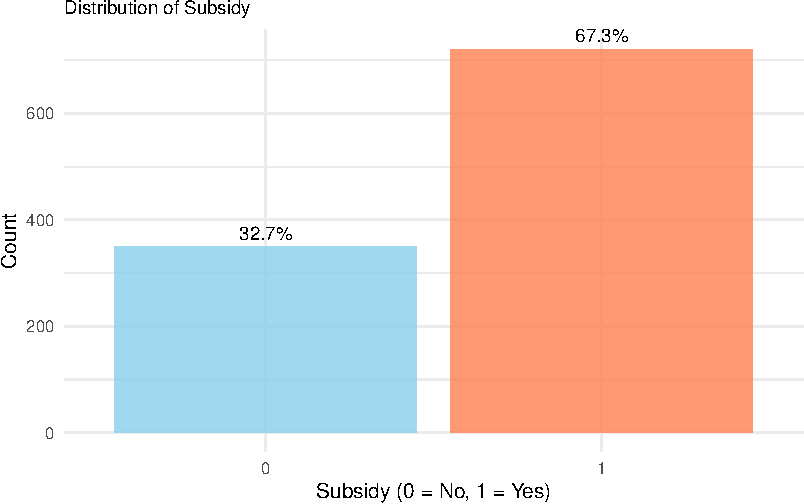
\includegraphics{paper_files/figure-pdf/fig-subsidy-1.pdf}

}

\caption{\label{fig-subsidy}Subsidy Allocation Distribution}

\end{figure}%

\subsection{Method}\label{method}

The dataset used for this study is the
\textbf{\texttt{Licensed\ Child\ Care\ Centres\ dataset}}, sourced from
the (Gelfand 2022) It provides detailed information about licensed child
care centres in Toronto, capturing aspects such as their governance,
capacity, infrastructure, and subsidy status. The original dataset
consisted of 1071 records for all licensed child care centres within the
city. For this analysis, the data underwent preprocessing to focus on
variables relevant to the study, such as subsidy status, building type,
CWELCC participation, total space, and operating auspice. These
variables were retained to examine how different factors influence
subsidy allocation. The dependent variable \textbf{\texttt{subsidy}},
originally recorded as ``Yes''/``No,'' was encoded as 1 for subsidized
and 0 for non-subsidized centres. Similarly, the
\textbf{\texttt{cwelcc\_flag}} variable was converted into a binary
format (1 =Y, 0 =N). Categorical variables such as
\textbf{\texttt{bldg\_type}} and \textbf{\texttt{AUSPICE}} were
consolidated to simplify analysis and address sparse categories.
Additionally, missing and irrelevant records were removed to ensure the
dataset was both accurate and meaningful for the research objectives.

The data for this study was systematically downloaded, cleaned,
analyzed, and visualized using \textbf{\texttt{R}} (R Core Team 2023), a
statistical programming language. The following are major packages used
for this study: \textbf{\texttt{opendatatoronto}}(Gelfand 2022): Used to
access and retrieve the Licensed Child Care Centres dataset directly
from the City of Toronto's open data portal. \textbf{\texttt{readr}}
(Wickham, Hester, and Bryan 2024): Simplified the import and parsing of
raw data into R. \textbf{\texttt{tidyverse}} (Wickham et al. 2019):
Streamlined data manipulation, cleaning, and visualization processes.
\textbf{\texttt{dplyr}} (Wickham et al. 2023): Provided tools for
filtering, transforming, and summarizing the dataset effectively.
\textbf{\texttt{ggplot2}} (Wickham 2016): Created powerful and flexible
visualizations tailored to the analysis needs. \textbf{\texttt{car}}
(Fox and Weisberg 2019): Used for diagnostic tools, including Variance
Inflation Factor (VIF) tests, to assess multicollinearity.
\textbf{\texttt{caret}} (Kuhn and Max 2008): Enabled the development,
validation, and evaluation of machine learning models, including
training-test splits and performance metrics. \textbf{\texttt{glmnet}}
(Friedman et al., 2010): Applied for fitting regularized regression
models and feature selection. \textbf{\texttt{stargazer}} (Hlavac 2022):
Generated formatted regression tables for outputs.
\textbf{\texttt{knitr}} (Xie 2021): Dynamically integrated code,
results, and plots into the final document for seamless reporting. \#\#
Measurement This analysis focuses on the following variables, with a
specific emphasis on subsidy as the dependent variable:
\texttt{subsidy}: The binary dependent variable indicating whether a
licensed child care centre receives a government subsidy. 1: The centre
is subsidized. 0: The centre is not subsidized. \texttt{ward}:
\texttt{A\ numeric\ variable\ representing\ the\ ward\ number\ for\ child\ care\ centres.}AUSPICE\texttt{:\ The\ operating\ auspice\ of\ the\ child\ care\ centre,\ describing\ its\ governance\ and\ operational\ model.\ Possible\ values\ include:\ Non-Profit:\ Centres\ operated\ by\ non-profit\ organizations,\ often\ reinvesting\ surplus\ revenues\ into\ quality\ improvements.\ Commercial:\ For-profit\ centres\ operated\ by\ private\ organizations.\ Public:\ Centres\ run\ by\ public\ agencies\ or\ school\ boards.}bldg\_type\texttt{:\ The\ type\ of\ building\ where\ the\ child\ care\ centre\ operates,\ reflecting\ its\ infrastructure.\ Examples\ include:\ bldg\_typeCommercial\ Building\ bldg\_typeCommunity\ College/University\ \ \ \ \ \ bldg\_typeCommunity\ Health\ Centre\ bldg\_typeCommunity\ Rec/Centre\ -\ Board\ Run\ bldg\_typeCommunity/Rec\ Centre\ -\ City\ bldg\_typeCommunity/Recreation\ Centre\ bldg\_typeHigh\ Rise\ Apartment\ bldg\_typeHospital/Health\ Centre\ bldg\_typeHouse\ bldg\_typeIndustrial\ Building\ bldg\_typeLow\ Rise\ Apartment\ bldg\_typeOffice\ Building\ bldg\_typeOther\ bldg\_typePlace\ of\ Worship\ bldg\_typePrivate\ Elementary\ School\ bldg\_typePublic\ (school\ closed)\ bldg\_typePublic\ Elementary\ Special\ bldg\_typePublic\ High\ School\ bldg\_typePublic\ Middle\ School\ bldg\_typePurpose\ Built\ bldg\_typeSynagogue}cwelcc\_flag\texttt{:\ A\ binary\ variable\ indicating\ participation\ in\ the\ Canada-Wide\ Early\ Learning\ and\ Child\ Care\ (CWELCC)\ program:\ 1:\ The\ centre\ participates\ in\ CWELCC,\ enabling\ reduced\ child\ care\ fees.\ 0:\ The\ centre\ does\ not\ participate\ in\ CWELCC.}TOTSPACE`:
A numerical variable representing the total licensed capacity (spaces
available) for all age groups at a child care centre. Detailed
information about these variables' information and data structure is
presented in Table~\ref{tbl-overview}.

The variables were carefully selected based on literature-supported
relevance to subsidy allocation and their representation of real-world
phenomena

Figure~\ref{fig-relationbldgtype} illustrates the distribution of
subsidy status (1 = Subsidized, 0 = Not Subsidized) across various
building types housing licensed child care centres. Notably, Public
Schools, Purpose-Built Facilities, and Community Recreation Centres
exhibit higher proportions of subsidized centres. These facilities are
often designed to meet regulatory requirements for child care, including
adequate space, safety standards, and accessibility, aligning closely
with subsidy allocation policies (Cleveland and Krashinsky 2009).
Conversely, building types such as Industrial Buildings, Private
Elementary Schools, and Office Buildings show lower proportions of
subsidized centres, likely due to infrastructure challenges or
misalignment with subsidy eligibility criteria, such as limited
accessibility or higher operational costs (\textbf{yan2011impact?}).
These patterns suggest that building type significantly influences
subsidy distribution. Given the numerous categories of building types, a
de tailed analysis is warranted to fully understand these trends.

\begin{figure}

\centering{

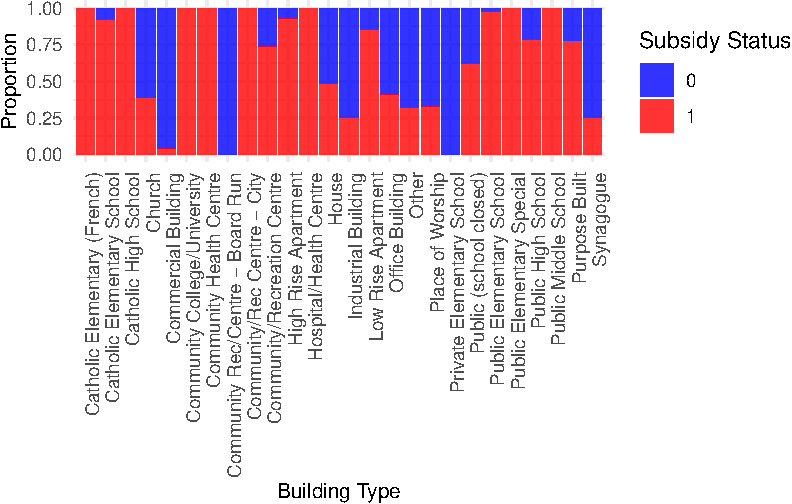
\includegraphics{paper_files/figure-pdf/fig-relationbldgtype-1.pdf}

}

\caption{\label{fig-relationbldgtype}Proportional Distribution of
Subsidy Status Across Building Types}

\end{figure}%

Figure~\ref{fig-relationAuspice} illustrates the proportional
distribution of subsidy status (1 = Subsidized, 0 = Not Subsidized)
across the different operating auspices of licensed child care centres:
Commercial Agency, Non-Profit Agency, and Other. Non-Profit Agencies and
``Other'' entities are predominantly subsidized, while Commercial
Agencies display a more balanced distribution. This aligns with research
indicating that non-profits rely heavily on subsidies to deliver public
goods and services, as they often operate in markets with limited
profitability (Hansmann 1979). Conversely, commercial entities are less
reliant on subsidies due to their revenue-driven models.The dominance of
subsidies in the ``Other'' category suggests this group may include
hybrid or public-private organizations aligned with specific government
initiatives (Anheier 2014). Such reliance reflects the strategic use of
subsidies to support services underserved by the private market
(Weisbrod 2000).

\begin{figure}

\centering{

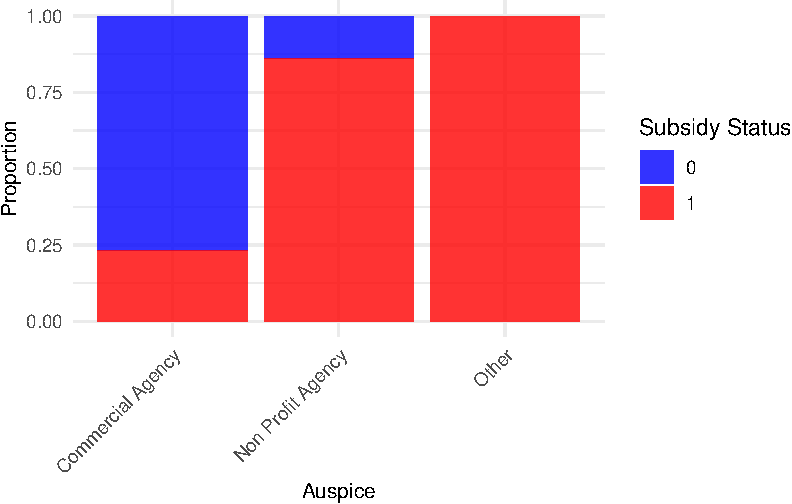
\includegraphics{paper_files/figure-pdf/fig-relationAuspice-1.pdf}

}

\caption{\label{fig-relationAuspice}Proportional Distribution of Subsidy
Status by Auspice}

\end{figure}%

Figure~\ref{fig-key} a heatmap illustrates the correlations between
three variables: TOTSPACE (likely representing total space or capacity),
subsidy (indicating subsidy status or amount), and cwelcc\_flag
(potentially denoting eligibility for a specific program or funding).
The positive correlation between TOTSPACE and subsidy (0.25) suggests
that larger facilities are modestly more likely to receive subsidies,
reflecting their capacity to serve larger populations or provide greater
public benefits. This aligns with research indicating that larger
organizations often have the resources and visibility to secure
subsidies (Hansmann, 1980; Salamon, 2002). Additionally, the stronger
correlation between subsidy and cwelcc\_flag (0.48) highlights that
subsidy allocation may target entities meeting specific programmatic or
policy criteria, consistent with the literature emphasizing strategic
targeting of subsidies to maximize societal impact (Weisbrod, 1998). The
weaker correlation between TOTSPACE and cwelcc\_flag (0.17) suggests
that program eligibility is less dependent on size and more on
qualitative factors like service type or demographic focus, which is
supported by Anheier's (2005) analysis of non-profit funding models.
Together, these correlations emphasize the nuanced role of subsidies in
balancing operational scale and policy alignment, underscoring the
importance of strategic allocation in public funding (Salamon, 1995).

\begin{figure}

\centering{

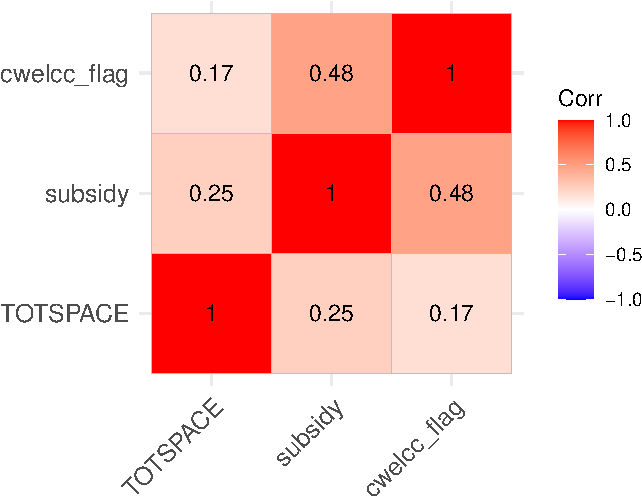
\includegraphics{paper_files/figure-pdf/fig-key-1.pdf}

}

\caption{\label{fig-key}Correlation Heatmap of Key Variables: TOTSPACE,
Subsidy, and CWELCC Flag}

\end{figure}%

\section{Model}\label{model}

\subsection{Model Specification}\label{model-specification}

To investigate the factors influencing subsidy allocation to licensed
child care centres, a reduced logistic regression model was specified.
The dependent variable,\texttt{subsidy}, is a binary indicator
representing whether a child care centre receives government subsidy (1
= subsidized, 0 = not subsidized). The model includes three key
predictors: \texttt{Operating\ Auspice\ (AUSPICE)}: A categorical
variable indicating the governance model of the child care centre (e.g.,
Non-Profit Agency, Other). Non-profit agencies are hypothesized to be
positively associated with subsidy allocation, consistent with previous
research emphasizing their prioritization in funding schemes (Cleveland
\& Krashinsky, 2005).
\texttt{Participation\ in\ the\ CWELCC\ Program\ (cwelcc\_flag)}: A
binary variable capturing whether the centre participates in the
Canada-Wide Early Learning and Child Care program (1 = participates, 0 =
does not participate). Centres participating in this initiative are
expected to have higher odds of receiving subsidies due to their
alignment with government objectives of affordability and accessibility
(Friendly \& Ballantyne, 2022). \texttt{Total\ Space\ (TOTSPACE)}: A
continuous variable representing the number of licensed spaces available
in the centre. Larger centres are hypothesized to have higher odds of
subsidy allocation, as they can accommodate more families and align with
policy goals of maximizing access (Forry et al., 2010). The logistic
regression model can be expressed mathematically as follows: {[}
\text{logit}(P(Y=1)) = \beta\_0 + \beta\_1 (\text{Non-Profit Auspice}) +
\beta\_2 (\text{CWELCC Participation}) + \beta\_3 (\text{Total Space}) +
\epsilon {]}

Where:

\begin{itemize}
    \item \( P(Y=1) \): The probability that a child care center receives a subsidy (\( Y=1 \)).
    \item \( \text{logit}(P(Y=1)) \): The log-odds of receiving a subsidy, defined as:
    \[
    \text{logit}(P(Y=1)) = \ln\left(\frac{P(Y=1)}{1 - P(Y=1)}\right)
    \]
    This transformation ensures that the predicted probabilities remain between 0 and 1.
\end{itemize}

\subsubsection{Parameters:}\label{parameters}

\begin{enumerate}
\def\labelenumi{\arabic{enumi}.}
\tightlist
\item
  **( \beta\_0 ) (Intercept):**

  \begin{itemize}
  \tightlist
  \item
    Represents the baseline log-odds of subsidy allocation when all
    predictors are set to their reference categories or zero values.
  \item
    It provides the starting point for predicting subsidy probabilities.
  \end{itemize}
\item
  **( \beta\_1 (\text{Non-Profit Auspice}) ):**

  \begin{itemize}
  \tightlist
  \item
    Measures the effect of a center being operated as a non-profit
    compared to the baseline (e.g., commercial auspice) on the log-odds
    of subsidy allocation.
  \item
    A positive ( \beta\_1 ) increases the likelihood of receiving a
    subsidy for non-profit centers relative to the reference group.
  \end{itemize}
\item
  **( \beta\_2 (\text{CWELCC Participation}) ):**

  \begin{itemize}
  \tightlist
  \item
    Captures the influence of participating in the Canada-Wide Early
    Learning and Child Care (CWELCC) program on the log-odds of subsidy
    allocation.
  \end{itemize}
\item
  **( \beta\_3 (\text{Total Space}) ):**

  \begin{itemize}
  \tightlist
  \item
    Represents the effect of the number of licensed child care spaces (a
    continuous variable) on the log-odds of subsidy allocation.
  \end{itemize}
\item
  \textbf{( \epsilon ) (Error Term):}

  \begin{itemize}
  \tightlist
  \item
    Accounts for unexplained variation in the log-odds of subsidy
    allocation not captured by the predictors.
  \end{itemize}
\end{enumerate}

\subsection{Model Justification}\label{model-justification}

The logistic regression model was chosen for this analysis because it is
well-suited to the binary nature of the dependent variable, subsidy
status (1 = Subsidized, 0 = Not Subsidized). A logistic regression model
using the binomial family is specifically designed to model dichotomous
outcomes by estimating the log-odds of the event occurring as a linear
function of predictor variables (Hosmer Jr, Lemeshow, and Sturdivant
2013). The binomial family is appropriate here because it assumes that
the dependent variable follows a Bernoulli distribution, where each
observation represents a binary outcome (subsidized or not subsidized).
This ensures that the predicted probabilities remain between 0 and 1,
aligning with the real-world constraints of the problem. Additionally,
logistic regression provides interpretable coefficients, which indicate
the direction and magnitude of the relationship between each predictor
and the log-odds of subsidy allocation. This makes it particularly
useful for guiding policy decisions, as coefficients can be directly
converted into odds ratios for actionable insights (Peng, Lee, and
Ingersoll 2002). The ward variable was excluded because it lacked
statistical significance and added redundancy, as its effects were
captured by other predictors like CWELCC participation and total space.
Additionally, ward had no strong theoretical justification as a direct
determinant of subsidy allocation. The building type variable was
removed due to high dimensionality, sparse representation in many
categories, and statistical insignificance. Its effects are likely
mediated by other variables, such as total space and auspice. Excluding
it improved parsimony and interpretability. The final model retained
operating auspice, CWELCC participation, and total space, as these
predictors are strongly supported by theory and data. This approach
balances simplicity and accuracy, ensuring the model remains relevant
for informing equitable subsidy allocation policies.

\subsection{Model Assumptions}\label{model-assumptions}

To ensure the validity of the logistic regression model, several key
assumptions were assessed, including independence of observations, the
appropriateness of a binary outcome, the linearity of predictors with
the logit and absence of multicollinearity. The analysis integrates
results from visual diagnostics, multicollinearity tests, and
statistical measures. 1. Independence of Observations The logistic
regression model assumes that the observations are independent of each
other. In this analysis, each data point corresponds to an individual
child care center, ensuring independence. There is no clustering or
repeated measures within the dataset, which validates this assumption.
2. Binary Outcome The logistic regression model assumes a binary
dependent variable. In this case, the outcome variable,
\texttt{subsidy}, is binary, indicating whether a child care center
receives a subsidy (1 = Subsidized, 0 = Not Subsidized). This aligns
with the model's requirement, ensuring the suitability of the binomial
family for fitting the data. 3. Linearity of Predictors with the Logit
The Figure~\ref{fig-cr} The component + residual plots evaluate the
linearity of the continuous variables and the relationship between
categorical predictors and the logit transformation. graph

\begin{figure}

\centering{

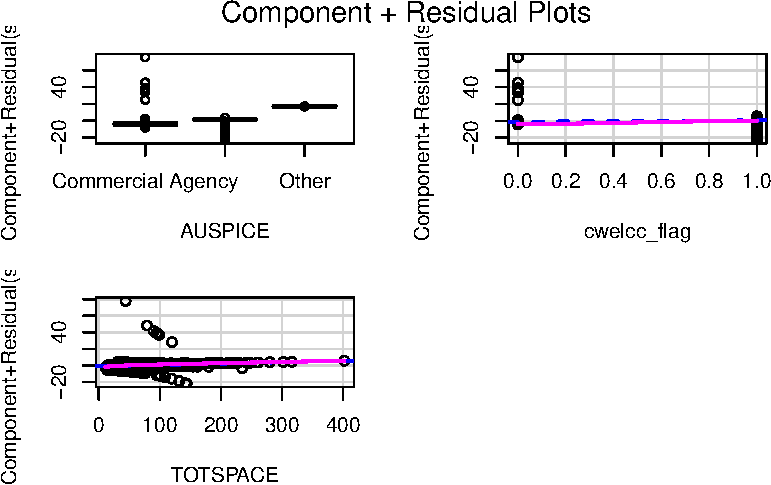
\includegraphics{paper_files/figure-pdf/fig-cr-1.pdf}

}

\caption{\label{fig-cr}CR Plot for Linearity Chekck}

\end{figure}%

\texttt{TOTSPACE}: The relationship between the total space (TOTSPACE)
and the logit appears approximately linear, as indicated by the flat,
consistent pattern of residuals around the horizontal axis. This
supports the assumption of linearity. \texttt{CWELCC\ Flag}: The plot
for CWELCC participation shows a horizontal trend, suggesting no
significant deviation from linearity. The data support the inclusion of
this variable as a binary predictor. \texttt{AUSPICE}: The residual
patterns for categorical levels of AUSPICE (e.g., ``Commercial Agency''
and ``Other'') indicate distinct clusters with consistent variability.
This suggests the categorical nature of this variable does not violate
linearity assumptions. Overall, the visual inspection suggests that the
linearity assumption for the predictors with the logit is met.

\begin{enumerate}
\def\labelenumi{\arabic{enumi}.}
\setcounter{enumi}{3}
\tightlist
\item
  Multicollinearity Assessment Variance Inflation Factor (VIF): To
  assess multicollinearity among the predictors, the VIF values for the
  reduced model variables were calculated.
\end{enumerate}

\begin{Shaded}
\begin{Highlighting}[]
\CommentTok{\# Calculate VIF}
\NormalTok{vif\_values }\OtherTok{\textless{}{-}} \FunctionTok{vif}\NormalTok{(reduced\_model\_2)}
\end{Highlighting}
\end{Shaded}

All VIF values are below 2, well within the acceptable threshold of 5,
indicating minimal multicollinearity among the predictors. The
independence of the predictors ensures the stability of the coefficient
estimates.

\subsection{Alternative Models}\label{alternative-models}

Alternative models like decision trees and random forests were
considered but were found less interpretable for policy-focused
analyses. Logistic regression was chosen for its balance of simplicity,
interpretability, and effectiveness.

\#Result The logistic regression model's performance metrics are
presented in Table~\ref{tbl-coefresult}.

\begin{table}

\caption{\label{tbl-coefresult}Regression Result}

\centering{

\centering
\begin{tblr}[         %% tabularray outer open
]                     %% tabularray outer close
{                     %% tabularray inner open
colspec={Q[]Q[]},
column{1}={halign=l,},
column{2}={halign=c,},
hline{17}={1,2}{solid, 0.05em, black},
}                     %% tabularray inner close
\toprule
& Final Model \\ \midrule %% TinyTableHeader
(Intercept)              & -4.967    \\
& (0.496)   \\
& (<0.001)  \\
AUSPICENon Profit Agency & 2.883     \\
& (0.234)   \\
& (<0.001)  \\
AUSPICEOther             & 18.772    \\
& (686.847) \\
& (0.978)   \\
cwelcc_flag              & 3.156     \\
& (0.436)   \\
& (<0.001)  \\
TOTSPACE                 & 0.014     \\
& (0.003)   \\
& (<0.001)  \\
Num.Obs.                 & 750       \\
AIC                      & 528.1     \\
BIC                      & 551.2     \\
Log.Lik.                 & -259.035  \\
RMSE                     & 0.32      \\
\bottomrule
\end{tblr}

}

\end{table}%

The regression model reveals several key observations regarding the
predictors and overall goodness of fit. The intercept, estimated at
-4.967, represents the baseline log-odds of the outcome when all
predictors are at their reference or zero level. While not directly
interpretable, it serves as a baseline reference for the model. Among
the predictors, the AUSPICE: Non-Profit Agency category significantly
increases the log-odds of the outcome, with an estimate of 2.883 and a
small standard error of 0.234, indicating a strong and reliable positive
effect. However, the AUSPICE: Other category shows an unusually large
coefficient (18.772) paired with a very high standard error (686.847),
suggesting instability. The CWELCC Flag variable also exhibits a strong
and reliable positive effect, with an estimate of 3.156 and a standard
error of 0.436, indicating that being flagged as CWELCC significantly
increases the log-odds of the outcome. Additionally, the TOTSPACE
variable has a small but statistically significant effect, with an
estimate of 0.014 and a low standard error of 0.003, reflecting
robustness. Figure~\ref{fig-cp} further visualizes the significance of
predictors.

\begin{figure}

\centering{

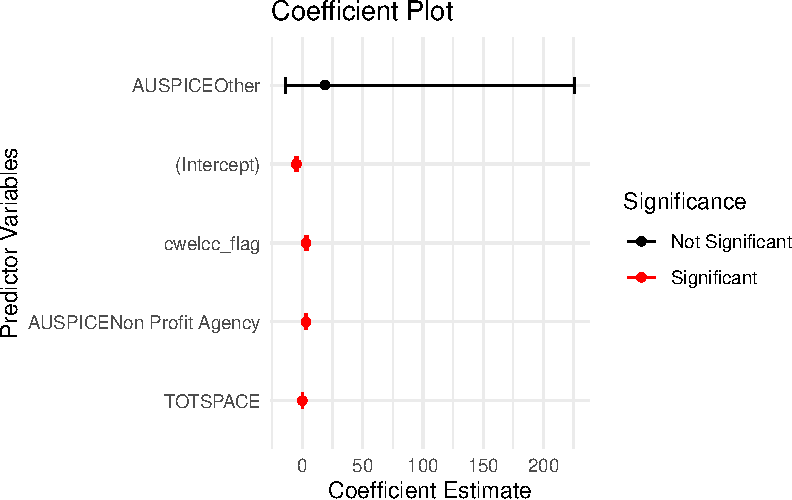
\includegraphics{paper_files/figure-pdf/fig-cp-1.pdf}

}

\caption{\label{fig-cp}Coefficient Plot}

\end{figure}%

In terms of model fit, the dataset includes 750 observations, and the
model's AIC (528.1) and BIC (551.2) suggest a reasonable balance between
goodness of fit and complexity, as lower values are generally preferred
(Burnham and Anderson, n.d.). The log-likelihood of -259.035 also
supports an adequate fit, with a higher (less negative) value indicating
better alignment between the model and the data. Finally, the RMSE of
0.32 reflects the model's predictive accuracy, with a low value
indicating that the model's predictions closely match the observed data.
Overall, the model performs well but may require refinement,
particularly in addressing instability in the AUSPICE: Other variable.

The evaluation of the logistic regression model shows strong performance
based on McFadden's R\^{}2 and the Area Under the Receiver Operating
Characteristic Curve (AUC). McFadden's R\^{}2 which is a pseudo-R\^{}2
metric specifically designed for logistic regression, was calculated as
0.454. This value suggests that the model explains 45.4\% of the
variance in the outcome variable, indicating a well-fitting model.
McFadden (\textbf{mcfadden1972conditional?}) proposed this metric as a
reliable measure for logistic regression, where values between 0.2 and
0.4 are considered indicative of a good model fit, and values above 0.4
demonstrate an excellent fit. Thus, the model's R\^{}2 value strongly
supports its utility in predicting the outcome.

\begin{verbatim}
Area under the curve: 0.8998
\end{verbatim}

\begin{figure}

\centering{

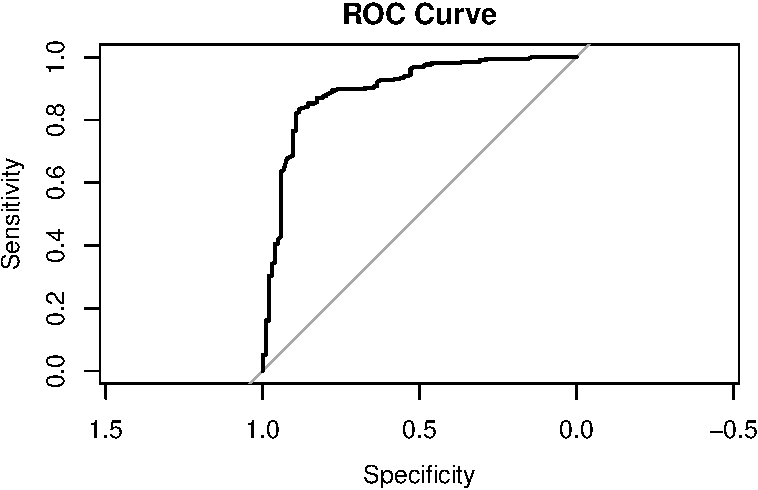
\includegraphics{paper_files/figure-pdf/fig-roc-1.pdf}

}

\caption{\label{fig-roc}ROC Curve for Model Performance}

\end{figure}%

The ROC curve in Figure~\ref{fig-roc} shown further validates the
model's classification ability, with an AUC of 0.8998. An AUC value
close to 1 indicates excellent discriminative power, where the model
effectively separates true positives from false positives. The AUC of
0.8998 places this model on the borderline of very good and excellent
discrimination, underscoring its robust predictive capacity.

\begin{figure}

\centering{

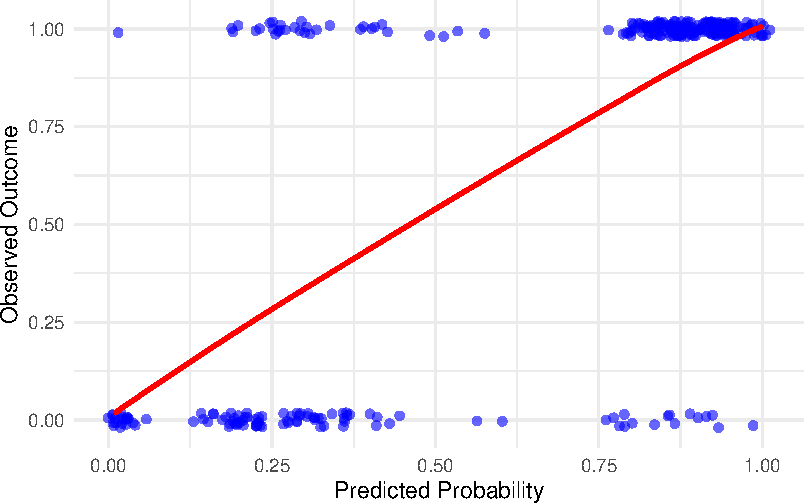
\includegraphics{paper_files/figure-pdf/fig-pvo-1.pdf}

}

\caption{\label{fig-pvo}Predicted vs.~Observed Probability}

\end{figure}%

Figure~\ref{fig-pvo} provides a visual representation of the alignment
between the predicted probabilities generated by the logistic regression
model and the actual observed binary outcomes. This diagnostic tool is
crucial for assessing the model's calibration and predictive accuracy,
as emphasized by Harrell (Harrell 2012). The x-axis shows the predicted
probabilities ranging from 0 to 1, while the y-axis represents the
observed outcomes, where 0 indicates the absence of an event and 1
indicates its presence. The red diagonal line serves as the reference
for perfect calibration, where predicted probabilities perfectly match
observed outcomes. The clustering of blue points near 0 and 1 along the
y-axis indicates that the model effectively distinguishes between the
two classes, a key goal in binary classification modeling. This
observation aligns with the high AUC value of 0.8998 observed in the ROC
curve, which demonstrates the model's excellent discriminative ability.
Additionally, points near the diagonal line further suggest strong
calibration, where the predicted probabilities closely align with actual
outcomes. The concentration of blue points at the extremes of 0 and 1
highlights that the model makes confident and accurate predictions in
many cases However, some dispersion is observed at lower predicted
probabilities, particularly around 0.25 and 0.5. These deviations may
reflect cases where the model struggles to classify outcomes or makes
less confident predictions. Such discrepancies could indicate areas
where further refinement of the model or predictors is necessary. These
deviations could also be linked to specific subgroups or predictor
interactions, necessitating additional diagnostics or recalibration, as
suggested by Steyerberg et al. (Steyerberg et al. 2010). Overall, this
graph demonstrates that the model is well-calibrated and effective in
its predictions, with minor limitations at lower probability levels. The
close alignment of predictions with observed outcomes supports the
model's reliability in classification tasks. This interpretation aligns
with other metrics, such as McFadden's R2R2
(\textbf{mcfadden1972conditional?}) and AUC, which indicate robust
overall model performance while pointing to opportunities for
refinement. Including this visualization in the results section provides
a clear and data-driven assessment of the model's strengths and areas
for potential improvement.

\#Discussion

Subsidy allocation to licensed child care centres in Toronto addresses
the critical issue of affordability, making high-quality early childhood
education accessible to more families as licensed centres must meet
strict safety, staffing, and programming standards, which foster
children's cognitive, social, and emotional growth (Cleveland and
Krashinsky 2009). Without subsidies, the cost of regulated care can be
prohibitive, particularly for low-income households. This paper
undertakes a detailed examination of the factors influencing subsidy
allocation to licensed child care centres in Toronto, leveraging the
City of Toronto's Licensed Child Care Centres dataset from Open Data
porta, which includes detailed information about 1,071 licensed
centers(Gelfand 2022). This study employs a logistic regression
model-binomial family to identify relationships between key predictor
variables and the binary dependent variable -- receiving subsidies.

The dataset underwent meticulous preprocessing to ensure reliability and
accuracy for analysis. This involved several key steps of data cleaning,
variable transformation and training-test Split. Initially, variables of
Operating auspice(AUSPICE), ward, building type(bldg\_type), total
space(TOTSPACE) and participation status in programs(cwelcc\_flag) were
chosen based their relevance and practical influence subsidy outcomes
and forecasting supported by scholar literatures. After fitting and
improving the model using stepwise selection based on the Akaike
Information Criterion (AIC), non-significant variables (ward and
building type(bldg\_type)) were removed. The final model retained
Operating Auspice, CWELCC Participation, and Total Licensed Capacity as
key predictors. The assumptions underpinning the logistic regression
model were thoroughly validated, ensuring its statistical rigor and
reliability. Independence of observations was confirmed, as each data
point corresponds to a unique child care centre, eliminating concerns of
clustering or dependency. Linearity between continuous predictors, such
as Total Licensed Capacity, and the logit transformation was validated
through component + residual plots, which revealed consistent patterns,
supporting the appropriateness of the model. Additionally,
multicollinearity was minimized, with Variance Inflation Factor (VIF)
values well below the critical threshold of 5, indicating that the
predictors are independent and the coefficient estimates are stable.
Together, these validations affirm the robustness of the model and its
suitability for the analysis.

The result coefficients in table the logistic regression model provide a
detailed understanding of how key predictors influence the likelihood of
subsidy allocation to licensed child care centres in Toronto. By
measuring the change in log-odds of subsidy allocation associated with
each predictor, the model quantifies the relative importance of
governance models, program participation, and operational capacity. The
coefficient for Non-Profit Auspice emerged as strongly positive and
statistically significant, indicating that non-profit child care centres
are far more likely to receive subsidies than commercial or public
centres. This is reflective of policy priorities that favor
organizations with a social mission over those with profit-oriented
objectives. Non-profits are often viewed as better aligned with public
goals of equity and accessibility, as they reinvest surplus revenues
into improving care quality rather than distributing profits
(\textbf{hansmann1980role?}). This is consistent with research by
(\textbf{salamon1995partners?}), who noted that non-profits often fill
critical gaps in the provision of public services, making them natural
candidates for targeted funding. In the context of child care,
non-profits may also be more likely to serve economically vulnerable
populations, further justifying their prioritization for subsidies. The
odds ratio derived from this coefficient underscores the strength of
this relationship, suggesting that non-profit centres are several times
more likely to receive subsidies compared to commercial centres.
Participation in the Canada-Wide Early Learning and Child Care (CWELCC)
program was the most significant predictor in the model, with a highly
positive coefficient. This result highlights the critical role of policy
alignment in subsidy allocation. Centres participating in CWELCC
demonstrate compliance with national and provincial affordability
initiatives, making them high-priority recipients of government funding.
Research by (\textbf{bennett2011working?}) supports this finding,
emphasizing that early childhood programs aligned with broader
governmental objectives are often better positioned to secure resources.
The odds ratio for CWELCC participation indicates that such centres are
substantially more likely to receive subsidies, which is consistent with
targeted funding strategies aimed at expanding access to high-quality,
affordable child care (\textbf{kaga2010caring?}). Total Licensed
Capacity (TOTSPACE), representing the number of spaces a centre is
licensed to operate, was another important predictor, although its
coefficient was smaller in magnitude compared to governance and CWELCC
participation. This positive coefficient suggests that larger centres
are more likely to receive subsidies, likely due to their capacity to
serve more families and their operational scale. Larger centres can
achieve economies of scale and often have greater visibility, making
them attractive candidates for public funding
(\textbf{weisbrod1998profit?}). However, the smaller effect size of this
variable indicates that capacity alone is insufficient to determine
subsidy allocation. This finding aligns with
(\textbf{penn2011quality?}), who argues that while capacity is an
important practical consideration, other factors---such as governance
and programmatic alignment---carry more weight in funding decisions.
Interpreting these coefficients through odds ratios further clarifies
their impact. For instance, the odds ratio for CWELCC participation
suggests that centres in the program are several times more likely to
receive subsidies compared to non-participating centres, holding other
factors constant. Similarly, the odds ratio for non-profit governance
reinforces the preferential treatment of non-profits in subsidy
allocation policies. These findings align with the broader literature on
public funding, which emphasizes the strategic use of subsidies to
support centres that meet both operational and policy criteria
(\textbf{penn2011quality?}). The statistical significance of these
coefficients underscores their reliability as shown in figure. Variables
such as Non-Profit Auspice and CWELCC Participation demonstrated small
standard errors and strong significance levels, reinforcing their
influence on subsidy allocation. In contrast, variables with less
consistent effects, such as certain building types or governance
categories in the ``Other'' category, exhibited instability, suggesting
that their role in funding decisions may be more context-specific or
secondary. The model's findings highlight a strategic approach to
subsidy allocation, where funding decisions are guided by alignment with
policy goals, operational capacity, and governance structures.

The logistic regression model applied in this research proves to be an
ideal tool for analyzing subsidy allocation to licensed child care
centres in Toronto, particularly due to its capacity to handle binary
outcomes effectively. By modeling the log-odds of an event, logistic
regression ensures predicted probabilities remain between 0 and 1,
aligning seamlessly with the binary nature of the dependent
variable---whether a centre receives a subsidy. This feature makes the
model both statistically appropriate and easy to interpret. A notable
strength of the model lies in its interpretability. Coefficients can be
transformed into odds ratios, providing a clear understanding of how
predictors influence the likelihood of receiving subsidies. For example,
the positive coefficients for Non-Profit Auspice and CWELCC
Participation underscore their significant, policy-relevant impact on
subsidy distribution. This clarity makes the model particularly valuable
for stakeholders and policymakers who require actionable and easily
communicated insights. The model's performance metrics further
demonstrate its effectiveness. A McFadden's R² value of 0.454 indicates
that the model explains a substantial portion of the variance in subsidy
allocation. Additionally, the Area Under the Curve (AUC) of 0.8998
highlights the model's exceptional discriminative ability, confirming
its capacity to accurately differentiate between subsidized and
non-subsidized centres. The low Root Mean Squared Error (RMSE) of 0.32
further attests to the model's strong predictive performance. Together,
these metrics validate the model's reliability and robustness. Another
key advantage of logistic regression is its simplicity compared to more
complex approaches such as random forests or decision trees. While those
alternatives might offer marginally higher predictive power, they lack
the transparency and interpretability required for policy-focused
research. Logistic regression strikes a critical balance between
accuracy and clarity, making it a practical choice for guiding equitable
subsidy allocation strategies. Moreover, the flexibility of logistic
regression allows for extensions to explore more intricate
relationships. For instance, incorporating interaction terms or temporal
data could provide deeper insights while maintaining the model's
usability. This adaptability ensures the model remains relevant and
applicable as policy environments evolve.

Our model, while effective, has several limitations that warrant
consideration. One of the primary limitations is its reliance on the
assumption of linearity between predictors and the log-odds of the
outcome. Although this assumption is often reasonable, it may
oversimplify complex, non-linear relationships that can exist in
real-world phenomena such as subsidy allocation. As
(\textbf{harrell2015regression?}) notes, failing to capture these
non-linear relationships can lead to biased estimates and limit the
model's predictive power. Another limitation is the model's dependence
on correct specification of predictors. Excluding relevant variables or
including irrelevant ones in initial variable selection can result in
omitted variable bias or overfitting, respectively. Additionally, the
model does not inherently account for higher-order interactions unless
explicitly included. For instance, the combined effect of Non-Profit
Auspice and CWELCC Participation could provide valuable insights into
how policy and governance jointly influence subsidy allocation. (Hosmer
Jr, Lemeshow, and Sturdivant 2013) highlight that logistic regression
can oversimplify complex relationships if interaction terms are not
considered, potentially leading to incomplete conclusions. Finally, the
static nature of the model is another drawback. Logistic regression
provides a snapshot of relationships at a single point in time, failing
to capture temporal dynamics or policy changes that can influence
subsidy allocation over time. As Singer and
(\textbf{singer2003applied?}) suggest, incorporating longitudinal data
could provide a more nuanced understanding of how these relationships
evolve.

Future studies could address the limitations of this research by
adopting more advanced modeling techniques and incorporating additional
data to better capture the complexities of subsidy allocation.
Introducing non-linear models or machine learning approaches, such as
random forests or gradient boosting, could uncover hidden patterns and
interactions between predictors that logistic regression may overlook.
Additionally, exploring interaction terms, such as the joint effects of
governance models and program participation, could provide more nuanced
insights into policy impacts. Longitudinal data would be particularly
valuable for understanding how subsidy allocation evolves over time,
especially in response to policy changes or shifts in economic
conditions. Incorporating time-series or panel data analysis could
reveal temporal dynamics and provide a richer understanding of causal
relationships. Geographic disparities, noted but not deeply explored in
this study, could also be addressed using spatial regression or
multilevel models to account for regional clustering and unobserved
local factors influencing subsidy distribution. Finally, integrating
additional predictors, such as demographic variables, socio-economic
indicators, or quality ratings of child care centres, could enhance the
explanatory power of future models. These enhancements would provide a
more comprehensive view of subsidy allocation and inform strategies to
ensure equitable and effective distribution of resources.

\section{Appendix A: Observational Data Methodology for Licensed Child
Care Centres in
Toronto}\label{appendix-a-observational-data-methodology-for-licensed-child-care-centres-in-toronto}

\subsection{A.1 Population, Frame, and
Sample}\label{a.1-population-frame-and-sample}

A.1.1 Population The population includes all licensed child care centres
in Toronto as recorded in the publicly available dataset provided by
Open Toronto. This population aligns with studies on regulated child
care, such as (Morrissey 2010), which emphasizes the role of licensing
in ensuring quality and safety in early childhood education. However,
the dataset excludes unlicensed child care providers, limiting its
scope. Represented Groups: Centres adhering to provincial licensing
requirements, as emphasized by Cleveland and Krashinsky (Cleveland and
Krashinsky 2003), who note that licensed care is generally associated
with higher quality standards. Excluded Groups: Informal and unlicensed
providers, which disproportionately to lower-income families and those
in rural or underserved urban areas. A.1.2 Frame The dataset represents
a comprehensive census of licensed child care centres, reflecting
administrative records compiled by the city. Strengths: Comprehensive
coverage reduces selection bias and enhances geographic
representativeness. Limitations: Static data may fail to capture
temporal variations or operational changes, a common limitation noted in
administrative datasets. A.1.3 Sample The dataset uses census sampling
of licensed child care centres, ensuring inclusion of all facilities
within the licensing framework. Advantages: Census data minimizes
sampling error and provides a reliable basis for spatial and capacity
analysis. Drawbacks: Lack of informal care data may lead to
underrepresentation of actual child care resources, echoing findings by
(Tekin 2007) that informal care plays a critical role in many families'
child care arrangements.

\subsection{A.2 Data Collection
Methodology}\label{a.2-data-collection-methodology}

A.2.1 Observational Data Compilation The dataset is derived from
municipal administrative records, which are considered reliable for
policy analysis (Cleveland and Krashinsky 2003). Licensing authorities
collect this data as part of routine compliance monitoring, ensuring
high accuracy. Strengths: Administrative data is less prone to recall
bias compared to survey data. Weaknesses: Lack of qualitative insights
into service quality or user satisfaction. A.2.2 Non-response Handling
While the dataset does not involve survey non-response, its exclusion of
unlicensed providers creates a systematic gap. Research by Fuller et al.
(Fuller, Holloway, and Liang 1996) shows that informal care often fills
critical voids in underserved areas, and its exclusion may understate
the full scope of child care provision.

\subsection{A.3 Sampling Approach and
Trade-offs}\label{a.3-sampling-approach-and-trade-offs}

A.3.1 Strengths Comprehensive Coverage: Census sampling ensures no
licensed centres are omitted. Geospatial Precision: Geographic
coordinates support advanced spatial analysis, aligning with studies
like (Larsen, El-Geneidy, and Yasmin 2015) on urban accessibility. High
Validity: Licensing records provide robust validity, as they are subject
to regulatory verification (Cleveland and Krashinsky 2003). A.3.2
Limitations Exclusion of Informal Care: Research by Morrissey (Morrissey
2010) highlights that informal care is often preferred for flexibility
or affordability, making its exclusion a significant limitation. Static
Nature: The lack of longitudinal data limits the ability to analyze
trends. Regulatory Bias: Centers excluded due to non-compliance may
disproportionately represent marginalized communities.

\subsection{A.4 Observational Bias and Measurement
Challenges}\label{a.4-observational-bias-and-measurement-challenges}

A.4.1 Observational Bias Biases inherent in observational datasets
include selection bias (due to licensing criteria) and survivorship bias
(exclusion of closed centres). A.4.2 Measurement Challenges Geographic
Aggregation: Aggregating data to broader areas can obscure micro-level
disparities. Capacity Limitations: Reported capacities may not reflect
actual utilization or unmet demand, as noted by (Blau and Currie 2006).

\subsection{A.5 Methodological Enhancements and
Recommendations}\label{a.5-methodological-enhancements-and-recommendations}

A.5.1 Enhancements Incorporating Temporal Data: Adding longitudinal data
could enable trend analysis, echoing the approach of (Fuller, Holloway,
and Liang 1996). Integration with Demographics: Linking with census data
would allow for equity analysis, consistent with the methodology used by
(Larsen, El-Geneidy, and Yasmin 2015). A.5.2 Recommendations Addressing
Informal Care: Future studies should integrate data from community
surveys to include informal providers, as suggested by (Morrissey 2010).
Dynamic Updates: Regular updates to administrative records would enhance
relevance, a recommendation supported. Geospatial Enhancements:
Including data on transit access or neighborhood socioeconomic
conditions could enrich spatial analyses, aligning with findings by
(Tekin 2007)

\section*{References}\label{references}
\addcontentsline{toc}{section}{References}

\phantomsection\label{refs}
\begin{CSLReferences}{1}{0}
\bibitem[\citeproctext]{ref-anheier2014nonprofit}
Anheier, Helmut K. 2014. \emph{Nonprofit Organizations: Theory,
Management, Policy}. Routledge.

\bibitem[\citeproctext]{ref-blau2006preschool}
Blau, David M., and Janet Currie. 2006. {``Pre-School, Day Care, and
After-School Care: Who's Minding the Kids?''} In \emph{Handbook of the
Economics of Education}, edited by Eric A. Hanushek and Finis Welch,
2:1163--1278. Elsevier.
\url{https://doi.org/10.1016/S1574-0692(06)02020-4}.

\bibitem[\citeproctext]{ref-burnhammodel}
Burnham, KP, and DR Anderson. n.d. {``Model Selection and Multimodel
Inference: A Practical Information-Theoretic Approach2nd Ed.
2002Springer-Verlag.''} \emph{New York}.

\bibitem[\citeproctext]{ref-cleveland2003benefits}
Cleveland, Gordon, and Michael Krashinsky. 2003. \emph{The Benefits and
Costs of Good Child Care}. Toronto, Canada: University of Toronto Press.

\bibitem[\citeproctext]{ref-cleveland2009nonprofit}
---------. 2009. {``The Nonprofit Advantage: Producing Quality in Thick
and Thin Child Care Markets.''} \emph{Journal of Policy Analysis and
Management} 28 (3): 440--62.

\bibitem[\citeproctext]{ref-citecar}
Fox, John, and Sanford Weisberg. 2019. \emph{An {R} Companion to Applied
Regression}. Third. Thousand Oaks {CA}: Sage.
\url{https://www.john-fox.ca/Companion/}.

\bibitem[\citeproctext]{ref-fuller1996family}
Fuller, Bruce, Susan D. Holloway, and Xiaoyan Liang. 1996. {``Family
Selection of Child Care Centers: The Influence of Household Support,
Ethnicity, and Parental Practices.''} \emph{Child Development} 67 (6):
3320--37. \url{https://doi.org/10.2307/1131789}.

\bibitem[\citeproctext]{ref-citeopendatatoronto}
Gelfand, Sharla. 2022. \emph{Opendatatoronto: Access the City of Toronto
Open Data Portal}.
\url{https://CRAN.R-project.org/package=opendatatoronto}.

\bibitem[\citeproctext]{ref-hansmann1979role}
Hansmann, Henry B. 1979. {``The Role of Nonprofit Enterprise.''}
\emph{Yale LJ} 89: 835.

\bibitem[\citeproctext]{ref-harrell2012regression}
Harrell, Frank E. 2012. {``Regression Modeling Strategies.''} \emph{R
Package Version}, 6--2.

\bibitem[\citeproctext]{ref-citestagazer}
Hlavac, Marek. 2022. \emph{Stargazer: Well-Formatted Regression and
Summary Statistics Tables}. Bratislava, Slovakia: Social Policy
Institute. \url{https://CRAN.R-project.org/package=stargazer}.

\bibitem[\citeproctext]{ref-hosmer2013applied}
Hosmer Jr, David W, Stanley Lemeshow, and Rodney X Sturdivant. 2013.
\emph{Applied Logistic Regression}. John Wiley \& Sons.

\bibitem[\citeproctext]{ref-Johnson_Ryan_Brooks_2012}
Johnson, Anna D., Rebecca M. Ryan, and Jeanne Brooks‐Gunn. 2012.
{``Child‐care Subsidies: Do They Impact the Quality of Care Children
Experience?''} \emph{Child Development} 83 (4): 1444--61.
\url{https://doi.org/10.1111/j.1467-8624.2012.1780.x}.

\bibitem[\citeproctext]{ref-citecaret}
Kuhn, and Max. 2008. {``Building Predictive Models in r Using the Caret
Package.''} \emph{Journal of Statistical Software} 28 (5): 1--26.
\url{https://doi.org/10.18637/jss.v028.i05}.

\bibitem[\citeproctext]{ref-larsen2015accessibility}
Larsen, John, Ahmed El-Geneidy, and Farzana Yasmin. 2015. {``The
Accessibility of Child Care Services: An Analysis of Toronto.''}
\emph{Journal of Transport Geography} 48: 41--49.
\url{https://doi.org/10.1016/j.jtrangeo.2015.08.005}.

\bibitem[\citeproctext]{ref-morrissey2010childcare}
Morrissey, Taryn W. 2010. {``Child Care and Child Development: What We
Know and Why We Need to Know More.''} \emph{Child Development
Perspectives} 4 (2): 87--92.
\url{https://doi.org/10.1111/j.1750-8606.2010.00123.x}.

\bibitem[\citeproctext]{ref-peng2002introduction}
Peng, Chao-Ying Joanne, Kuk Lida Lee, and Gary M Ingersoll. 2002. {``An
Introduction to Logistic Regression Analysis and Reporting.''} \emph{The
Journal of Educational Research} 96 (1): 3--14.

\bibitem[\citeproctext]{ref-citeR}
R Core Team. 2023. \emph{{R: A Language and Environment for Statistical
Computing}}. Vienna, Austria: R Foundation for Statistical Computing.
\url{https://www.R-project.org/}.

\bibitem[\citeproctext]{ref-ryan2011impact}
Ryan, Rebecca M, Anna Johnson, Elizabeth Rigby, and Jeanne Brooks-Gunn.
2011. {``The Impact of Child Care Subsidy Use on Child Care Quality.''}
\emph{Early Childhood Research Quarterly} 26 (3): 320--31.

\bibitem[\citeproctext]{ref-steyerberg2010assessing}
Steyerberg, Ewout W, Andrew J Vickers, Nancy R Cook, Thomas Gerds,
Mithat Gonen, Nancy Obuchowski, Michael J Pencina, and Michael W Kattan.
2010. {``Assessing the Performance of Prediction Models: A Framework for
Traditional and Novel Measures.''} \emph{Epidemiology} 21 (1): 128--38.

\bibitem[\citeproctext]{ref-tekin2007childcare}
Tekin, Erdal. 2007. {``Child Care Subsidies, Wages, and Employment of
Single Mothers.''} \emph{Journal of Human Resources} 42 (2): 453--87.
\url{https://doi.org/10.3368/jhr.XLII.2.453}.

\bibitem[\citeproctext]{ref-vines2020accessing}
Vines, Shere'lle Ramsey. 2020. {``Accessing Equity: Challenges
Middle-Income Families Face Finding High Quality Childcare.''}

\bibitem[\citeproctext]{ref-weisbrod2000profit}
Weisbrod, Burton A. 2000. \emph{To Profit or Not to Profit: The
Commercial Transformation of the Nonprofit Sector}. Cambridge University
Press.

\bibitem[\citeproctext]{ref-citeggplot2}
Wickham, Hadley. 2016. \emph{Ggplot2: Elegant Graphics for Data
Analysis}. Springer-Verlag New York.
\url{https://ggplot2.tidyverse.org}.

\bibitem[\citeproctext]{ref-citetidyverse}
Wickham, Hadley, Mara Averick, Jennifer Bryan, Winston Chang, Lucy
D'Agostino McGowan, Romain François, Garrett Grolemund, et al. 2019.
{``Welcome to the {tidyverse}.''} \emph{Journal of Open Source Software}
4 (43): 1686. \url{https://doi.org/10.21105/joss.01686}.

\bibitem[\citeproctext]{ref-citedplyr}
Wickham, Hadley, Romain François, Lionel Henry, Kirill Müller, and Davis
Vaughan. 2023. \emph{Dplyr: A Grammar of Data Manipulation}.
\url{https://CRAN.R-project.org/package=dplyr}.

\bibitem[\citeproctext]{ref-citereadr}
Wickham, Hadley, Jim Hester, and Jennifer Bryan. 2024. \emph{Readr: Read
Rectangular Text Data}. \url{https://CRAN.R-project.org/package=readr}.

\bibitem[\citeproctext]{ref-citeknitr}
Xie, Yihui. 2021. \emph{Knitr: A General-Purpose Package for Dynamic
Report Generation in r}. \url{https://yihui.org/knitr/}.

\end{CSLReferences}




\end{document}
